%% pscc2026_template.tex, slightly modified by Florin Capitanescu on 2025/03/15
%% based on the version V1.1, 2019/03/11 provided by Mario Paolone
%% This is a Latex template to prepare submissions for the PSCC 2026 conference.
%% The template demonstrates the use of the class IEEEtran4PSCC.cls and is mostly
%% based on the file bare_conf.tex (V1.4a) by Michael Shell.

%%*************************************************************************
%% Legal Notice:
%% This code is offered as-is without any warranty either expressed or
%% implied; without even the implied warranty of MERCHANTABILITY or
%% FITNESS FOR A PARTICULAR PURPOSE!
%% User assumes all risk.
%% In no event shall PSCC or any contributor to this code be liable for
%% any damages or losses, including, but not limited to, incidental,
%% consequential, or any other damages, resulting from the use or misuse
%% of any information contained here.
%%
%% All comments are the opinions of their respective authors and are not
%% necessarily endorsed by the PSCC.
%%
%% This work is distributed under the LaTeX Project Public License (LPPL)
%% ( http://www.Latex-project.org/ ) version 1.3, and may be freely used,
%% distributed and modified. A copy of the LPPL, version 1.3, is included
%% in the base LaTeX documentation of all distributions of LaTeX released
%% 2003/12/01 or later.
%% Retain all contribution notices and credits.
%% ** Modified files should be clearly indicated as such, including  **
%% ** renaming them and changing author support contact information. **
%%
%% File list of work: pscc2026_template.tex, IEEEtran4PSCC.cls
%%*************************************************************************


% *** Authors should verify (and, if needed, correct) their LaTeX system  ***
% *** with the testflow diagnostic prior to trusting their LaTeX platform ***
% *** with production work.                 ***


\documentclass{IEEEtran4PSCC}
% The automatically selected options are the format (US letter) and conference mode.


% Some very useful LaTeX packages include:
% (uncomment the ones you want to load)
% *** MISC UTILITY PACKAGES ***
%
%\usepackage{ifpdf}
% Heiko Oberdiek's ifpdf.sty is very useful if you need conditional
% compilation based on whether the output is pdf or dvi.
% usage:
% \ifpdf
%   % pdf code
% \else
%   % dvi code
% \fi
% The latest version of ifpdf.sty can be obtained from:
% http://www.ctan.org/tex-archive/macros/Latex/contrib/oberdiek/
% Also, note that IEEEtran.cls V1.7 and later provides a builtin
% \ifCLASSINFOpdf conditional that works the same way.
% When switching from Latex to pdfLatex and vice-versa, the compiler may
% have to be run twice to clear warning/error messages.

% *** CITATION PACKAGES ***
%
%\usepackage{cite}
% cite.sty was written by Donald Arseneau
% V1.6 and later of IEEEtran pre-defines the format of the cite.sty package
% \cite{} output to follow that of IEEE. Loading the cite package will
% result in citation numbers being automatically sorted and properly
% 'compressed/ranged'. e.g., [1], [9], [2], [7], [5], [6] without using
% cite.sty will become [1], [2], [5]--[7], [9] using cite.sty. cite.sty's
% \cite will automatically add leading space, if needed. Use cite.sty's
% noadjust option (cite.sty V3.8 and later) if you want to turn this off
% such as if a citation ever needs to be enclosed in parenthesis.
% cite.sty is already installed on most LaTeX systems. Be sure and use
% version 5.0 (2009-03-20) and later if using hyperref.sty.
% The latest version can be obtained at:
% http://www.ctan.org/tex-archive/macros/Latex/contrib/cite/
% The documentation is contained in the cite.sty file itself.


% *** GRAPHICS RELATED PACKAGES ***
%
\ifCLASSINFOpdf
   \usepackage[pdftex]{graphicx}
  % declare the path(s) where your graphic files are
  % \graphicspath{{../pdf/}{../jpeg/}}
  % and their extensions so you won't have to specify these with
  % every instance of \includegraphics
  % \DeclareGraphicsExtensions{.pdf,.jpeg,.png}
\else
  % or other class option (dvipsone, dvipdf, if not using dvips). graphicx
  % will default to the driver specified in the system graphics.cfg if no
  % driver is specified.
   \usepackage[dvips]{graphicx}
  % declare the path(s) where your graphic files are
  % \graphicspath{{../eps/}}
  % and their extensions so you won't have to specify these with
  % every instance of \includegraphics
  % \DeclareGraphicsExtensions{.eps}
\fi
% graphicx was written by David Carlisle and Sebastian Rahtz. It is
% required if you want graphics, photos, etc. graphicx.sty is already
% installed on most LaTeX systems. The latest version and documentation
% can be obtained at:
% http://www.ctan.org/tex-archive/macros/Latex/required/graphics/
% Another good source of documentation is 'Using Imported Graphics in
% LaTeX2e' by Keith Reckdahl which can be found at:
% http://www.ctan.org/tex-archive/info/epsLatex/
%
% Latex, and pdfLatex in dvi mode, support graphics in encapsulated
% postscript (.eps) format. pdfLatex in pdf mode supports graphics
% in .pdf, .jpeg, .png and .mps (metapost) formats. Users should ensure
% that all non-photo figures use a vector format (.eps, .pdf, .mps) and
% not a bitmapped formats (.jpeg, .png). IEEE frowns on bitmapped formats
% which can result in 'jaggedy'/blurry rendering of lines and letters as
% well as large increases in file sizes.
%
% You can find documentation about the pdfTeX application at:
% http://www.tug.org/applications/pdftex



% *** MATH PACKAGES ***
%
\usepackage[cmex10]{amsmath}
\usepackage{amsfonts,amssymb,amsthm}
\usepackage{xspace}
\usepackage[linktocpage=true,colorlinks=true,linkcolor=blue,citecolor=blue,urlcolor=blue]{hyperref}
\usepackage{cleveref}
% A popular package from the American Mathematical Society that provides
% many useful and powerful commands for dealing with mathematics. If using
% it, be sure to load this package with the cmex10 option to ensure that
% only type 1 fonts will utilized at all point sizes. Without this option,
% it is possible that some math symbols, particularly those within
% footnotes, will be rendered in bitmap form which will result in a
% document that can not be IEEE Xplore compliant!
%
% Also, note that the amsmath package sets \interdisplaylinepenalty to 10000
% thus preventing page breaks from occurring within multiline equations. Use:
%\interdisplaylinepenalty=2500
% after loading amsmath to restore such page breaks as IEEEtran.cls normally
% does. amsmath.sty is already installed on most LaTeX systems. The latest
% version and documentation can be obtained at:
% http://www.ctan.org/tex-archive/macros/Latex/required/amsLatex/math/





% *** SPECIALIZED LIST PACKAGES ***
%
% \usepackage{algorithmic}
% algorithmic.sty was written by Peter Williams and Rogerio Brito.
% This package provides an algorithmic environment fo describing algorithms.
% You can use the algorithmic environment in-text or within a figure
% environment to provide for a floating algorithm. Do NOT use the algorithm
% floating environment provided by algorithm.sty (by the same authors) or
% algorithm2e.sty (by Christophe Fiorio) as IEEE does not use dedicated
% algorithm float types and packages that provide these will not provide
% correct IEEE style captions. The latest version and documentation of
% algorithmic.sty can be obtained at:
% http://www.ctan.org/tex-archive/macros/Latex/contrib/algorithms/
% There is also a support site at:
% http://algorithms.berlios.de/index.html
% Also of interest may be the (relatively newer and more customizable)
% algorithmicx.sty package by Szasz Janos:
% http://www.ctan.org/tex-archive/macros/Latex/contrib/algorithmicx/




% *** ALIGNMENT PACKAGES ***
%
%\usepackage{array}
% Frank Mittelbach's and David Carlisle's array.sty patches and improves
% the standard LaTeX2e array and tabular environments to provide better
% appearance and additional user controls. As the default LaTeX2e table
% generation code is lacking to the point of almost being broken with
% respect to the quality of the end results, all users are strongly
% advised to use an enhanced (at the very least that provided by array.sty)
% set of table tools. array.sty is already installed on most systems. The
% latest version and documentation can be obtained at:
% http://www.ctan.org/tex-archive/macros/Latex/required/tools/


% IEEEtran contains the IEEEeqnarray family of commands that can be used to
% generate multiline equations as well as matrices, tables, etc., of high
% quality.




% *** SUBFIGURE PACKAGES ***
%\ifCLASSOPTIONcompsoc
%  \usepackage[caption=false,font=normalsize,labelfont=sf,textfont=sf]{subfig}
%\else
%  \usepackage[caption=false,font=footnotesize]{subfig}
%\fi
% subfig.sty, written by Steven Douglas Cochran, is the modern replacement
% for subfigure.sty, the latter of which is no longer maintained and is
% incompatible with some LaTeX packages including fixltx2e. However,
% subfig.sty requires and automatically loads Axel Sommerfeldt's caption.sty
% which will override IEEEtran.cls' handling of captions and this will result
% in non-IEEE style figure/table captions. To prevent this problem, be sure
% and invoke subfig.sty's 'caption=false' package option (available since
% subfig.sty version 1.3, 2005/06/28) as this is will preserve IEEEtran.cls
% handling of captions.
% Note that the Computer Society format requires a larger sans serif font
% than the serif footnote size font used in traditional IEEE formatting
% and thus the need to invoke different subfig.sty package options depending
% on whether compsoc mode has been enabled.
%
% The latest version and documentation of subfig.sty can be obtained at:
% http://www.ctan.org/tex-archive/macros/Latex/contrib/subfig/




% *** FLOAT PACKAGES ***
%
%\usepackage{fixltx2e}
% fixltx2e, the successor to the earlier fix2col.sty, was written by
% Frank Mittelbach and David Carlisle. This package corrects a few problems
% in the LaTeX2e kernel, the most notable of which is that in current
% LaTeX2e releases, the ordering of single and double column floats is not
% guaranteed to be preserved. Thus, an unpatched LaTeX2e can allow a
% single column figure to be placed prior to an earlier double column
% figure. The latest version and documentation can be found at:
% http://www.ctan.org/tex-archive/macros/Latex/base/


%\usepackage{stfloats}
% stfloats.sty was written by Sigitas Tolusis. This package gives LaTeX2e
% the ability to do double column floats at the bottom of the page as well
% as the top. (e.g., '\begin{figure*}[!b]' is not normally possible in
% LaTeX2e). It also provides a command:
%\fnbelowfloat
% to enable the placement of footnotes below bottom floats (the standard
% LaTeX2e kernel puts them above bottom floats). This is an invasive package
% which rewrites many portions of the LaTeX2e float routines. It may not work
% with other packages that modify the LaTeX2e float routines. The latest
% version and documentation can be obtained at:
% http://www.ctan.org/tex-archive/macros/Latex/contrib/sttools/
% Do not use the stfloats baselinefloat ability as IEEE does not allow
% \baselineskip to stretch. Authors submitting work to the IEEE should note
% that IEEE rarely uses double column equations and that authors should try
% to avoid such use. Do not be tempted to use the cuted.sty or midfloat.sty
% packages (also by Sigitas Tolusis) as IEEE does not format its papers in
% such ways.
% Do not attempt to use stfloats with fixltx2e as they are incompatible.
% Instead, use Morten Hogholm'a dblfloatfix which combines the features
% of both fixltx2e and stfloats:
%
% \usepackage{dblfloatfix}
% The latest version can be found at:
% http://www.ctan.org/tex-archive/macros/Latex/contrib/dblfloatfix/




% *** PDF, URL AND HYPERLINK PACKAGES ***
%
% \usepackage{url}
% url.sty was written by Donald Arseneau. It provides better support for
% handling and breaking URLs. url.sty is already installed on most LaTeX
% systems. The latest version and documentation can be obtained at:
% http://www.ctan.org/tex-archive/macros/Latex/contrib/url/
% Basically, \url{my_url_here}.




% *** Do not adjust lengths that control margins, column widths, etc. ***
% *** Do not use packages that alter fonts (such as psLatex).         ***
% There should be no need to do such things with IEEEtran.cls V1.6 and later.


% correct bad hyphenation here
\hyphenation{op-tical net-works semi-conduc-tor}



% Set footer
\makeatletter
\let\old@ps@headings\ps@headings
\let\old@ps@IEEEtitlepagestyle\ps@IEEEtitlepagestyle
\def\psccfooter#1{%
    \def\ps@headings{%
        \old@ps@headings%
        \def\@oddfoot{\strut\hfill#1\hfill\strut}%
        \def\@evenfoot{\strut\hfill#1\hfill\strut}%
    }%
    \def\ps@IEEEtitlepagestyle{%
        \old@ps@IEEEtitlepagestyle%
        \def\@oddfoot{\strut\hfill#1\hfill\strut}%
        \def\@evenfoot{\strut\hfill#1\hfill\strut}%
    }%
    \ps@headings%
}
\makeatother

\psccfooter{%
        \parbox{\textwidth}{\hrulefill \\ \small{24th Power Systems Computation Conference} \hfill \begin{minipage}{0.2\textwidth}\centering \vspace*{4pt} \includegraphics[scale=0.06]{PSCC_logo.png}\\\small{PSCC 2026} \end{minipage} \hfill \small{Limassol, Cyprus --- June 8-12, 2026}}%
}


\begin{document}
\title{
An Augmented Lagrangian Method on GPU for Security-Constrained AC Optimal Power Flow
}


%% To specify the authors when (number of affiliations <= 2)
% \author{
% \IEEEauthorblockN{Author n.1 Name per Affiliation A\\ Author n.2 Name per Affiliation A}
% \IEEEauthorblockA{(Affiliation A) Department Name of Organization \\
% Name of the organization, acronyms acceptable\\
% City, Country\\
% \{email author n.1, email author n.2\}@domain (if desired)}
% \and
% \IEEEauthorblockN{Author n.1 Name per Affiliation B\\ Author n.2 Name per Affiliation B}
% \IEEEauthorblockA{(Affiliation B) Department Name of Organization \\
% Name of the organization, acronyms acceptable\\
% City, Country\\
% \{email author n.1, email author n.2\}@domain (if desired)}
% }


%% To specify the authors when (number of affiliations > 2)
\author{\IEEEauthorblockN{François Pacaud\IEEEauthorrefmark{1},
Armin Nurkanović\IEEEauthorrefmark{2},
Anton Pozharskiy \IEEEauthorrefmark{2},
Alexis Montoison\IEEEauthorrefmark{3} and
Sungho Shin\IEEEauthorrefmark{4}}
\IEEEauthorblockA{\IEEEauthorrefmark{1} Centre Automatique et Systèmes\\
Mines Paris-PSL,
Paris, France\\ francois.pacaud@minesparis.psl.eu}
\IEEEauthorblockA{\IEEEauthorrefmark{2}
  Department of Microsystems Engineering (IMTEK) \\
  University of Freiburg, Germany}
\IEEEauthorblockA{\IEEEauthorrefmark{3} Mathematics and Computer Science Division \\
Argonne National Laboratory,
Lemont, IL, USA}
\IEEEauthorblockA{\IEEEauthorrefmark{4}
  Massachusetts Institute of Technology \\
Cambridge, Massachusetts, USA
}
}


% make the title area
\maketitle

% As a general rule, do not put math, special symbols or citations
% in the abstract
\begin{abstract}
  We present a new algorithm for solving large-scale security-constrained optimal power flow in polar form (AC-SCOPF). The method builds on Nonlinearly Constrained augmented Lagrangian (NCL), an augmented Lagrangian method in which the subproblems are solved using an interior-point method. NCL has two key advantages for large-scale SCOPF. First, NCL handles difficult problems such as infeasible ones or models with complementarity constraints. Second, the augmented Lagrangian term naturally regularizes the Newton linear systems within the interior-point method, enabling solution of the Newton systems with a pivoting-free factorization that can be efficiently parallelized on GPUs. We assess the performance of our implementation, called MadNCL, on large-scale corrective AC-SCOPFs, with complementarity constraints modeling the corrective actions. Numerical results show that MadNCL can solve AC-SCOPF with 500 buses and 256 contingencies fully on the GPU in less than 3 minutes, whereas Knitro takes more than 3 hours to find an equivalent solution.
\end{abstract}

\begin{IEEEkeywords}
  AC-SCOPF;
  Augmented Lagrangian method;
  Contingency screening;
  GPU acceleration;
  Nonlinear programming.
% The author shall provide up to 5 keywords (in alphabetical order) to help identify the major topics of the paper.
\end{IEEEkeywords}


% Use this to place sponsorships
\thanksto{\noindent Submitted to the 24th Power Systems Computation Conference (PSCC 2026).}


\section{Introduction}
\subsection{Motivation}
In transmission networks, the optimal dispatch is usually computed by solving
a security-constrained optimal power flow (SCOPF). The dispatch
minimizes a given criterion (costs or network losses) while considering
physical constraints (power flow, line flow limits) and the generators' capacities.
Furthermore, the dispatch should remain feasible
for a set of contingency scenarios corresponding to the loss of a line or a generator in the network ($N-1$ security criterion).
We refer to \cite{stott2005security,frank2016introduction} for comprehensive descriptions of the SCOPF problem.

The SCOPF is usually formulated as a large-scale linear program called the DC-SCOPF, whose size
grows linearly with the number of contingencies~\cite{alsac2002further}.
This comes at the price of linearizing the nonlinear physical constraints, diminishing the solution's accuracy~\cite{coffrin2012approximating}.
However, solving the AC-SCOPF with the original nonlinear formulation remains an open challenge,
and was the main motivation behind the recent GO competition~\cite{aravena2023recent}.
The issue with the nonlinear formulation is two-fold. First, the AC-SCOPF is a a huge-scale
nonlinear program, whose size is beyond the capacity of state-of-the-art nonlinear optimization solvers
like Ipopt or Knitro~\cite{wachter2006implementation,waltz2006interior,capitanescu2011state}.
Second, the complementarity constraints in the AC-SCOPF models are numerically
difficult to handle, and a tailored algorithm must be employed.
These complementarity constraints arise from the set of logical conditions
modeling the droop control and the PV/PQ switches constraining the recourse in the post-contingency state.
Complementarity constraints have been adopted early
on in power system computation, both for power flow~\cite{zhao2008pv,sundaresh2014modified,murray2015robust} and for optimal power flow~\cite{rosehart2005optimal}.
However, the AC-SCOPF reformulated with complementarity constraints yields a degenerate nonlinear program
coming with its own issues.

\subsection{Augmented Lagrangian method}

There exist numerous algorithms to solve mathematical programs with complementarity constraints (MPCCs) \cite{nurkanovic2024}.
For instance, the teams in the GO-competition handled the complementarity constraints
using active-set methods~\cite{curtis2023decomposition}, homotopy reformulations~\cite{gholami2023admm,petra2023surrogate} or an $\ell_1$-exact penalty reformulation~\cite{leyffer2006interior}.
The large-scale nature of AC-SCOPFs pushes algorithms to their limit, as the number
of complementarity constraints grows linearly with the number of contingencies.
To address this challenge, we propose to solve the AC-SCOPF with an augmented Lagrangian
method based on the Nonlinearly Constrained augmented Lagrangian (NCL)~\cite{ma2017stabilized,montoison2025madncl}. Algorithm NCL comes with three benefits for SCOPF problems:
(1) it can quickly detect local infeasibility (a common situation for AC-SCOPF)~\cite{chiche2016augmented},
(2) it is robust and can handle complementarity constraints~\cite{izmailov2012global},
(3) it has a structure favorable for GPU acceleration, as the Newton systems we obtain
in the algorithm can be solved efficiently in parallel without numerical pivoting~\cite{montoison2025madncl}.
MadNCL is a recent implementation of Algorithm NCL built on top of MadNLP, and supports
the solution of large-scale problems on the GPU using the linear solver NVIDIA cuDSS.
As such, MadNCL~\cite{montoison2025madncl} can be considered as an extension of our previous work investigating
the solution of large-scale optimal power flow (OPF) on the GPU with MadNLP~\cite{shin2024accelerating}.

% lien NCL two-stage ADMM

\subsection{Scope and contributions}
In this work, we analyze the performance of MadNCL~\cite{montoison2025madncl}
on large-scale AC-SCOPF instances formulated as MPCCs.
To the best of our knowledge, this is the first time an augmented Lagrangian-based algorithm is used to solve the corrective SCOPF formulated with complementarity constraints. We present numerical
experiments showing that MadNCL can accommodate well the complementarity constraints in the AC-SCOPF and
is effective at detecting infeasible problems --- a useful feature for contingency screening.
We detail how to deploy the computation on the GPU for faster solution time.
On the GPU, MadNCL evaluates the derivatives with ExaModels~\cite{shin2024accelerating} and solves the Newton systems with NVIDIA cuDSS.
We compare MadNCL with Artelys Knitro~\cite{waltz2006interior}, a state-of-the-art optimization
solver that supports the solution of MPCCs~\cite{leyffer2006interior}.


\section{Model}
In this section, we detail how to formulate the AC-SCOPF with complementarity constraints.
We adapt the formulation used in the GO competition~\cite{aravena2023recent}.
We denote by $K$ the number of contingencies, and refer to the base case by the index $k=0$.
We suppose the system has $n_b$ buses, $n_\ell$ lines and $n_g$ generators.
For $k=0, \cdots, K$, the voltage magnitudes and angles at buses are denoted by
$(v_b^k, \theta_b^k) \in \mathbb{R}^{n_b} \times \mathbb{R}^{n_b}$, the loads by $(p_{\ell}, q_\ell)$ and the active and reactive power generations by $(p_g^k, q_g^k) \in \mathbb{R}^{n_g} \times \mathbb{R}^{n_g}$.
For $(a, b) \in \mathbb{R}^2$, we say that $a$ complements $b$ if $a \geq 0$, $b \geq 0$
and $a b = 0$. The complementarity constraint is denoted by $0 \leq a \perp b \geq 0$.

\subsection{AC-OPF model}
We formulate the model using the classical polar formulation of the AC-OPF problem.
The variables in the base case and the contingencies have the following bounds,
for $k=0, 1,\cdots, K$,
\begin{equation}
  \begin{aligned}
  & \underline{p}_g \leq p_g^k \leq \overline{p}_g \; , \quad
  \underline{q}_g \leq q_g^k \leq \overline{q}_g \; , \\
  & \underline{v}_b \leq v_b^k \leq \overline{v}_b \; , \quad
  \underline{\theta}_b \leq \theta_b^k \leq \overline{\theta}_b \; .
  \end{aligned}
\end{equation}
The active and reactive power flow constraints at each bus are,
for $i=1, \cdots, n_b$:
\begin{equation*}
  \begin{aligned}
    & \sum_{j \in \mathcal{G}(i)} p_{g,j}^k - p_{\ell,i} - g_i^{sh} (v_{b,i}^k)^2 - \sum_{j \in \mathcal{N}(i)} p_{ij}^k = 0 \; , \\
    & \sum_{j \in \mathcal{G}(i)} q_{g,j}^k - q_{\ell,i} + b_i^{sh} (v_{b,i}^k)^2 - \sum_{j \in \mathcal{N}(i)} q_{ij}^k = 0 \; ,\\
    & \text{with, for all arcs $(i, j)$}, \\
    & p_{ij}^k = y_{1ij} (v_{b,i}^k)^2 - (y_{3ij} \cos(\Delta\theta_{ij}^k) + y_{4ij} \sin(\Delta\theta_{ij}^k))v_{b,i}^k v_{b,j}^k \;,  \\
    & q_{ij}^k = y_{2ij} (v_{b,i}^k)^2 + (y_{4ij} \cos(\Delta\theta_{ij}^k) - y_{3ij} \sin(\Delta\theta_{ij}^k)) v_{b,i}^k v_{b,j}^k\; ,
  \end{aligned}
\end{equation*}
with $\Delta\theta_{ij}^k := \theta_{b,i}^k - \theta_{b,j}^k$,
and $(y_{1ij}, y_{2ij}, y_{3ij}, y_{4ij})$ four coefficients associated to the physical
parameters of the line $(i,j)$.
The line current rating constraints are:
\begin{equation*}
  (p_{ij}^k)^2 + (q_{ij}^k)^2 \leq (\overline{\ell}_{ij}^k)^2 (v_{b,i}^k)^2 \; , \;
  \quad \forall (i, j) \; ,
\end{equation*}
with $\ell_{ij}^k$ the rate of line $(i, j)$ in contingency $k$ (equal to $0$ if the
line is removed in contingency $k$).


\subsection{Recourse constraints}
In SCOPF, the variation of the power production $p_g^k \in \mathbb{R}^{n_g}$ in contingency $k$
should reflect the behavior of the \emph{automatic generation control system}
(AGC, also known as droop control): the active power is used to regulate the
frequency in the post-contingency state. Given a participation factor
encoded as a vector $\alpha_g \in \mathbb{R}^{n_g}$, the power generation
in contingency $k$ is given by
\begin{equation}
  \label{eq:agc}
  p_g^k = \min\Big(\max\big( p_g^0 + \alpha_g \Delta^k , \; \underline{p}_g \big), \; \overline{p}_g \Big) \; ,
\end{equation}
where $\Delta^k \in \mathbb{R}$ is a variable encoding the power adjustment in contingency $k$
and $\underline{p}_g, \overline{p}_g$ are two vectors encoding the lower and upper bounds on the
active power generation.
The nonsmooth $\min$ and $\max$ operations clip $p_g^0 + \alpha_g \Delta^k$ to the bounds, and can be written as
a set of complementarity constraints~\cite{baumrucker2008mpec}: for non-negative $\pi_{g+}^k \geq 0$
and $\pi_{g-}^k \geq 0$ Equation~\eqref{eq:agc} is equivalent to,
for all $k=1, \cdots, K$,
\begin{equation}
  \label{eq:droopmpec}
  \begin{aligned}
    & \pi_{g+}^k - \pi_{g-}^k = p_{g}^k - (p_g^0 + \alpha_g \Delta) \; , \\
    & 0 \leq \pi_{g-}^k \perp \overline{p}_g - p_g^k \geq 0 \; , \\
    & 0 \leq \pi_{g+}^k \perp p_g^k - \underline{p}_g \geq 0 \; .
  \end{aligned}
\end{equation}
Similarly, the \emph{voltage control} keeps the voltage
magnitudes at the PV buses at their nominal values $v_{b}^k = v_{b}^0$ by injecting
or absorbing reactive power. However, if the reactive power production $q_g^k$ reaches
its lower $\underline{q}_g$ or upper limit $\overline{q}_g$, the bus is converted to a PQ bus and the voltage is allowed
to vary. The PV/PQ switches are modeled with a second set of complementarity constraints with,
for $\nu_{b-}^k \geq 0$ and $\nu_{b+}^k \geq 0$:
\begin{equation}
  \label{eq:pvpq}
  \begin{aligned}
    & \nu_{b+}^k - \nu_{b-}^k = v_b^k - v_b^0 \; ,\\
    & 0 \leq \nu_{b-}^k \perp \overline{q}_g - q_g^k \geq 0 \; , \\
    & 0 \leq \nu_{b+}^k \perp q_g^k - \underline{q}_g \geq 0 \; .
  \end{aligned}
\end{equation}
The corrective SCOPF modeling the recourse with \eqref{eq:droopmpec}
and \eqref{eq:pvpq} is a nonlinear program with complementarity
constraints. The MPCC formulation has been adopted throughout the GO
competition, and is described at length in \cite{aravena2023recent,curtis2023decomposition,gholami2023admm}.

\subsection{Optimization model}
We adapt the formulation of the AC-SCOPF used in \cite{frank2016introduction} to include the complementarity
constraints modeling the AGC~\eqref{eq:droopmpec} and the PV/PQ switches~\eqref{eq:pvpq}.
We note $u_0 = (p_g^0, v_{b,PV}^0)$ and $x_0 = (\theta_b^0, v_{b,PQ}^0, q_g^0)$ the control and the state in the base case,
and $u_k = (p_g^k, v_{b,PV}^k)$ and $x^k = (\theta_b^k, v_{b,PQ}^k, q_g^k, \Delta^k, \pi_g^k, \nu^k_b)$
the control and the state in contingency $k$. We define the AC-SCOPF problem as
\begin{equation}
  \label{eq:scopf}
  \begin{aligned}
    \min_{x, u} \; & f(x_0, u_0) \\
    \text{s.t.} \quad & g_0(x_0, u_0) = 0 \; , \;  h_0(x_0, u_0) \leq 0 \; , \\
                      & \forall k \in \{1,\cdots,K\} :\\
                            & g_k(u_0, x_k, u_k) = 0 \;, \;  h_k(x_k, u_k) \leq 0 \; , \\
                            & 0 \leq G(x_k, u_k) \perp H(x_k, u_k) \geq 0 \; ,
  \end{aligned}
\end{equation}
where $u = (u_0, u_1, \cdots, u_K)$, $x = (x_0, x_1, \cdots, x_K)$,
$f(\cdot)$ is the objective in the base case scenario,
$g_k(\cdot)$ encodes the power-flow constraints and the two linear constraints
in \eqref{eq:droopmpec} and \eqref{eq:pvpq}, $h_k(\cdot)$ the operational
constraints (line-flow and operational bounds) and $G(\cdot)$ and
$H(\cdot)$ are two functions encoding the
complementarity parts in \eqref{eq:droopmpec} and \eqref{eq:pvpq}.
In contrast to the formulation used by the GO-competition~\cite{aravena2023recent}, we do not
penalize the constraint violation in the objective using an $\ell_1$ penalty.

For a given base-case control $u_0$, the contingency $k$ is feasible if there is a solution
$(x_k, u_k)$ to the nonlinear system with complementarity constraints:
\begin{equation}
  \label{eq:screening}
  \left\{
  \begin{aligned}
    &  g_k(u_0, x_k, u_k) = 0 \; ,\;  h_k(x_k, u_k) \leq 0 \; , \\
    & 0 \leq G(x_k, u_k) \perp H(x_k, u_k) \geq 0 \; .
  \end{aligned}
  \right.
\end{equation}
The goal of \eqref{eq:scopf} is to find a base-case control $u_0$ such
that \eqref{eq:screening} is feasible for all the contingency $k=1,\cdots,K$.

\section{Mathematical programs with complementarity constraints}
The complementarity constraints complicate the solution of the problem \eqref{eq:scopf}.
As such, they are usually reformulated with binary variables using a big-M method,
leading to the formulation of a mixed-integer nonlinear program (MINLP). However,
the large-number of binary variables renders the MINLP quickly intractable.
Instead, we choose to address directly the complementarity constraints
and solve \eqref{eq:scopf} using an augmented Lagrangian method based on the algorithm NCL.
We detail the formulation of the SCOPF~\eqref{eq:scopf} as a mathematical
program with complementarity constraints (MPCC) in \S\ref{sec:mpcc:intro},
and discuss the associated first-order complementarity conditions in \S\ref{sec:mpcc:stationary}.
Classical solution methods are discussed in \S\ref{sec:mpcc:solution}.

\subsection{MPCC in vertical formulation}
\label{sec:mpcc:intro}
Upon introducing slack variables to reformulate the inequality constraints
and the nonlinear complementarity constraints in \eqref{eq:scopf}, we obtain
the equivalent MPCC in vertical form:
\begin{equation}
  \label{eq:mpcc}
  \begin{aligned}
    \min_{w \in \mathbb{R}^n} \; & \phi(w) \quad \text{s.t.} \quad \left\{
      \begin{aligned}
        & c(w) = 0 \; , w_0 \geq 0 \; , \\
        & 0 \leq w_1 \perp w_2 \geq 0 \; ,
      \end{aligned}
    \right.
  \end{aligned}
\end{equation}
with $w \in \mathbb{R}^n$ the variable aggregating the controls, states and slack variables
and $c: \mathbb{R}^n \to \mathbb{R}^m$ a function aggregating all the equality and inequality constraints
in \eqref{eq:scopf}.
We partition the decision variable as $w = (w_0, w_1, w_2) \in \mathbb{R}^{n-2p} \times
\mathbb{R}^p \times \mathbb{R}^p$ to isolate the variables contributing to the $p$ complementarity constraints.
For multipliers $(\lambda, \xi, \mu_1, \mu_2) \in \mathbb{R}^{m} \times \mathbb{R}^{n-2p} \times \mathbb{R}^p \times \mathbb{R}^p$, we define
the MPCC Lagrangian as
\begin{multline}
  \mathcal{L}^{\mathrm{MPCC}}(w, \lambda, \xi, \mu) = \phi(w) + \lambda^\top c(w) \\ - \xi^\top w_0 - \mu_1^\top w_1 - \mu_2^\top w_2 \; .
\end{multline}
The complementarity constraints in \eqref{eq:mpcc} state that for $i=1,\cdots,p$, $w_{1i} w_{2i} = 0$
and $(w_{1i}, w_{2i}) \geq 0$. As both variables appearing in the product are positive,
the complementarity constraints rewrite equivalently with inequality constraints as $w_{1i} w_{2i} \leq 0$
and $(w_{1i}, w_{2i}) \geq 0$ for $i=1,\cdots,p$: this alternative formulation
gives the best result when used in conjunction with an interior-point method~\cite{leyffer2006interior}.
Thus, a popular reformulation of~\eqref{eq:mpcc} is:
\begin{equation}
  \label{eq:mpccnlp}
  \begin{aligned}
    \min_{w \in \mathbb{R}^n} \; & \phi(w) \quad \text{s.t.} \quad
    \left\{
    \begin{aligned}
      & c(w) = 0 \; , \; w_0 \geq 0 \; , \\
      & (w_1, w_2) \geq 0 \; , \; W_1 W_2 e \leq 0 \; ,
    \end{aligned}
    \right.
  \end{aligned}
\end{equation}
where we have noted $W_1 = \text{diag}(w_1)$ and $W_2 = \text{diag}(w_2)$ with $e \in \mathbb{R}^p$
a vector of ones.
The Lagrangian for \eqref{eq:mpccnlp} is
\begin{multline}
  \mathcal{L}(w, \lambda, \xi, \nu) = \phi(w) + \lambda^\top c(w) \\ - \xi^\top w_0 - \nu_1^\top w_1 - \nu_2^\top w_2 + \nu_0^\top W_1 W_2 e \; .
\end{multline}
Problem~\eqref{eq:mpccnlp} is degenerate and the Mangasarian-Fromovitz constraint qualification (MFCQ)
fails for all feasible points. Indeed, suppose we have a single complementarity
constraint such that $(w_1, w_2) \geq 0$ and $w_1 w_2 \leq 0$. By definition, a feasible point $(w_1, w_2)$ satisfies
MFCQ if there exists a feasible direction $(d_1, d_2)$ such that $d_1 > 0$ if $w_1 = 0$, $d_2 > 0$ if
$w_2 = 0$ and $w_2 d_1 + w_1 d_2 < 0$. If $w_1 = 0$ and $w_2 > 0$, we get $d_1 > 0$ and $w_2 d_1 < 0$,
which is a contradiction as $w_2$ is positive. If the complementarity constraint
is biactive (both $w_1 = 0$ and $w_2 = 0$) the condition $w_2 d_1 + w_1 d_2 < 0$ cannot hold.
Hence MFCQ is not satisfied, and as a consequence the set of optimal multipliers $(\lambda, \nu)$ can be unbounded,
leading to potential numerical issues in
classical nonlinear programming solvers~\cite{leyffer2006interior}.

\subsection{First-order stationary conditions}
\label{sec:mpcc:stationary}
We note the feasible set of \eqref{eq:mpcc} as
\begin{equation*}
  \Omega = \{ w \in \mathbb{R}^n \; | \; c(w) = 0 \, , w_0 \geq 0 \; ,\; 0 \leq w_1 \perp w_2 \geq 0 \} \; .
\end{equation*}
For any feasible point $w \in \Omega$, we define the index sets
\begin{equation}
  \begin{aligned}
    \mathcal{I}_{+0}(w) = \{ i \in \{1, \cdots, p\} \; | \; w_{1,i} > 0 \, , \, w_{2,i} = 0 \} \;, \\
    \mathcal{I}_{0+}(w) = \{ i \in \{1, \cdots, p\} \; | \; w_{1,i} = 0 \, , \, w_{2,i} > 0 \} \;, \\
    \mathcal{I}_{00}(w) = \{ i \in \{1, \cdots, p\} \; | \; w_{1,i} = 0 \, , \, w_{2,i} = 0 \} \; .
  \end{aligned}
\end{equation}
% If $\mathcal{I}_{00}(w)$ is empty, we say $w$ satisfies \emph{strict complementarity}.
% A point $w \in \Omega$ is \emph{Bouligand-stationary}~\cite{scheel2000mathematical} if $d = 0$ solves the linear program
% with complementarity constraints (LPCC):
% \begin{equation}
%   \label{eq:stationarylpcc}
%   \begin{aligned}
%     \min_{d \in \mathbb{R}^n} \; & \; \nabla \phi(w)^\top d \\
%                                 & \nabla c_i(w)^\top d = 0 \;,\\
%                                 & d_{1,i} = 0 \;,\; & \forall i \in \mathcal{I}_{0+}(w), \\
%                                 & d_{2,i} = 0 \;,\; & \forall i \in \mathcal{I}_{+0}(w), \\
%                                 & 0 \leq d_{1,i} \perp d_{2,i} \geq 0 \;,\; & \forall i \in \mathcal{I}_{00}(w) \; .
%   \end{aligned}
% \end{equation}
The point $w \in \Omega$ satisfies \emph{strong stationarity}~\cite{scheel2000mathematical} if there exist
multipliers $(\lambda, \xi, \mu) \in \mathbb{R}^m \times \mathbb{R}^{2p}$ such that
\begin{equation}
  \label{eq:strongstationarity}
  \begin{aligned}
    & \nabla_w \mathcal{L}^{\mathrm{MPCC}}(w, \lambda, \xi, \mu) = 0 \; ,\\
    & c(w) = 0 \; , \; w_0 \geq 0 \; ,\\
    & w_{1,i} \geq 0 \; , \; \mu_{1,i} = 0 \;,\; w_{2, i} = 0 \;,\; \mu_{2,i} \in \mathbb{R} \;,\; \forall i \in \mathcal{I}_{+0}(w) \; , \\
    & w_{1,i} = 0 \; , \; \mu_{1,i} \in \mathbb{R} \;,\; w_{2, i} \geq 0 \;,\; \mu_{2,i} = 0 \;,\; \forall i \in \mathcal{I}_{0+}(w) \; , \\
    & w_{1,i} = 0 \; , \; \mu_{1,i} \geq 0 \;,\; w_{2, i} = 0 \;,\; \mu_{2,i} \geq 0 \;,\; \forall i \in \mathcal{I}_{00}(w) \; .
  \end{aligned}
\end{equation}
Conditions \eqref{eq:strongstationarity} are the KKT stationary solution of a relaxed nonlinear program~\cite{scheel2000mathematical} with no complementarity constraint.
If the relaxed nonlinear program satisfies Linear Independence Constraint Qualification (LICQ),
we say that MPCC-LICQ holds at $w \in \Omega$.
Our goal is to find a strong stationary solution for \eqref{eq:mpcc}.
% Every $w \in \Omega$ satisfying strong stationarity satisfies Bouligand stationarity~\cite{scheel2000mathematical}, with equivalence if MPCC-LICQ holds.


\subsection{Solution methods}
\label{sec:mpcc:solution}
The solution of MPCC~\eqref{eq:mpcc} has been widely studied since the 2000s.
\emph{Direct methods} solve Problem~\eqref{eq:mpccnlp} directly using
sequential quadratic programming (SQP) or an interior-point method (IPM)~\cite{fletcher2006local}.
\emph{Regularization methods} relax the degenerate terms in \eqref{eq:mpccnlp}
with a small parameter $\tau > 0$, such that the constraint $W_1 W_2 e \leq 0$
is reformulated as $W_1 W_2 e \leq \tau$. We obtain the so-called Scholtes
relaxation~\cite{scholtes2001convergence}: by driving the term $\tau$ to $0$ we recover the solution of the original MPCC~\eqref{eq:mpcc}.
\emph{Penalty-based methods} use an $\ell_1$-exact penalty to penalize the complementarity
constraints in the objective by adding a term $\tau w_1^\top w_2$, with a large-enough penalty $\tau >0$.
Assuming MPCC-LICQ, the $\ell_1$-exact penalty method converges to a strong-stationary solution $w \in \Omega$
\cite{ralph2004some}.
This is the method used in the solver Knitro~\cite{leyffer2006interior}.
In the next section, we interpret NCL as a mix of regularization and penalty-based methods.

\section{Augmented Lagrangian for MPCCs}
In this section, we present Algorithm NCL in \S\ref{sec:ncl:ncl} and
analyze the structure of the Newton systems in \S\ref{sec:ncl:newton}.
We show that NCL can solve the problem~\eqref{eq:mpccnlp} on the GPU.

\subsection{Algorithm NCL}
\label{sec:ncl:ncl}
The augmented Lagrangian method introduces a penalty $\rho^{(n)}$
and two multiplier estimates $(\lambda^{(n)}, \nu_0^{(n)}) \in \mathbb{R}^m \times \mathbb{R}^p$.
When the problem has a mix of equality and inequality constraints,
the augmented Lagrangian subproblem is:
\begin{equation}
  \label{eq:auglagsubpb}
  \min_{w \geq 0} \;  \mathcal{L}_\rho(w, \lambda^{(n)}, \nu^{(n)}_0)
\end{equation}
with $\mathcal{L}_\rho(w, \lambda^{(n)}, \nu^{(n)}_0) := \phi(w) + \frac{1}{2\rho^{(n)}} ( \| c(w) + \lambda^{(n)} \|^2 + \|\max\{ 0, W_1 W_2e + \nu_0^{(n)} \} \|^2 )$.
Upon finding appropriate multipliers estimates $(\lambda^{(n)}, \nu_0^{(n)})$ and penalty $\rho^{(n)}$,
the solution of \eqref{eq:auglagsubpb} converges to the solution of \eqref{eq:mpccnlp}~\cite{izmailov2012global}.
However, the augmented Lagrangian $\mathcal{L}_\rho(\cdot)$ comes with two issues:
the $\max$ term implies that the second-order derivatives are not continuous everywhere,
and even when it is defined, the Hessian $\nabla_{x x}^2 \mathcal{L}_\rho$ gets ill-conditioned as we increase the penalty $\rho$.

On its end, NCL is strictly equivalent to the classical augmented Lagrangian method,
but uses a nonlinearly constrained formulation in the subproblems.
NCL solves both problems by introducing two free regularization
variables $(r, t) \in \mathbb{R}^m \times \mathbb{R}^p$, and solves the equivalent subproblem:
\begin{equation}
  \label{eq:nclsubpb}
  \begin{aligned}
    \min_{w, r, t} \; & \;   \phi(w) + (\lambda^{(n)})^\top r  + (\nu_0^{(n)})^\top t +  \frac{\rho^{(n)}}{2}\|(r, t) \|^2  \; , \\
    \text{s.t.} \quad & c(w) - r = 0 \; , \\
                      & W_1 W_2 e \leq t  \; , \; w \geq 0 \; .
  \end{aligned}
\end{equation}
We emphasize that NCL treats \eqref{eq:mpccnlp} as a generic nonlinear program, and does not
apply any special treatment to the complementarity constraints. The regularization
$t$ plays the role of the Scholtes relaxation parameter (see \S\ref{sec:mpcc:solution})
and is penalized in the objective by the Augmented Lagrangian penalty.

We make a distinction between the {outer} and the {inner} iterations.
At a given outer iteration $n$, NCL solves \eqref{eq:nclsubpb}
with an interior-point method (IPM). The inner iterations refer to the IPM steps themselves.
Only the objective changes between two successive outer iterations, hence the IPM
can be efficiently warmstarted from the previous primal-dual solution.
Once Subproblem~\eqref{eq:nclsubpb} is solved, we update the augmented Lagrangian
parameters $(\rho^{(n)}, \lambda^{(n)}, \nu_0^{(n)})$ using the solution $(w^{n+1}, r^{n+1}, t^{n+1})$
and proceed to the next outer iteration.
For a given forcing sequence $\{\eta^{(n)}\}_n$, NCL uses the classical updates:
\begin{itemize}
  \item If $\|(r^{(n+1)}, t^{(n+1)})\|_\infty \leq \eta^{(n)}$, then
    \begin{equation*}
      \begin{aligned}
      & (\lambda^{(n+1)}, \nu_0^{(n+1)}) = (\lambda^{(n)}, \nu_0^{(n)}) + \rho^{(n)} (r^{(n+1)}, t^{(n+1)}) \; ,\\
      & \rho^{(n+1)} = \rho^{(n)} \; .
      \end{aligned}
    \end{equation*}
  \item Otherwise, set
    \begin{equation*}
      \lambda^{(n+1)} = \lambda^{(n)} \; , \;
      \nu_0^{(n+1)} = \nu_0^{(n)} \; , \;
      \rho^{(n+1)} = 10 \rho^{(n)} \; .
    \end{equation*}
\end{itemize}
We refer to \cite{montoison2025madncl} for a comprehensive description of the algorithm.
It has been proven in \cite{izmailov2012global} that the augmented Lagrangian
method converges to a strongly stationary solution $w \in \Omega$ of \eqref{eq:mpccnlp}
if MPCC-LICQ holds at $w$
and the sequence of multiplier estimates $\{\nu_0^n\}_n$ generated by the algorithm
has a bounded subsequence (this prevents the algorithm from converging to a spurious solution).

If the problem is infeasible, the penalty $\rho^{(n)}$ diverges to $+\infty$
and NCL iterates converge to a stationary solution of the \emph{feasibility problem}
\begin{equation}
  \label{eq:feaspb}
  \begin{aligned}
    \min_{w, r, t} \; & \; \|r\|^2 + \|t\|^2 \\
    \text{s.t.} \quad & c(w) - r = 0 \\
                      & (w_0, w_1, w_2) \geq 0 \; , \; W_1 W_2 e \leq t \;.
  \end{aligned}
\end{equation}
As discussed in \cite{izmailov2012global}, the augmented Lagrangian algorithm
can converge to a solution of \eqref{eq:feaspb} even if the original problem
is feasible: this is known caveat, and a similar situation can occur if we
replace the augmented Lagrangian by a $\ell_1$ exact penalty~\cite{leyffer2006interior}.
% By checking the respective values in the regularization variables $r$ and $t$,
% we can quickly assess which contingencies and constraints are rendering the SCOPF problem~\eqref{eq:scopf} infeasible.

\subsection{Newton systems}
\label{sec:ncl:newton}
The Karush-Kuhn-Tucker (KKT) stationary conditions for Subproblem~\eqref{eq:nclsubpb} are
\begin{equation}
  \label{eq:kktncl}
  \begin{aligned}
    & \nabla \phi(w) + \nabla c(w)^\top \lambda = 0\\
    & \lambda^{(n)} + \rho^{(n)} r - \lambda = 0 \\
    & \nu_0^{(n)} + \rho^{(n)} t - \nu = 0 \\
    & c(w) - r = 0 \\
    & 0 \leq w_0 \perp \xi \geq 0 \\
    & 0 \leq t - W_1 W_2 e \perp \nu_0 \geq 0 \\
    & 0 \leq w_1 \perp \nu_1 \geq 0 \; , \; 0 \leq w_2 \perp \nu_2 \geq 0 \; .
  \end{aligned}
\end{equation}
Upon introducing a slack $s := t - W_1 W_2e$, a primal-dual interior-point method
solves system~\eqref{eq:kktncl} for $(w, r, t, s, \lambda, \xi, \nu)$ using a Newton method. For a given
barrier parameter $\mu > 0$, the complementarity conditions in \eqref{eq:kktncl} are reformulated as
\begin{equation}
  W_0 \Xi = \mu e \; , \; S V_0 = \mu e \; , \; W_1 V_1 = \mu e \; , \; W_2 V_2 = \mu e \; ,
\end{equation}
with $\Xi = \text{diag}(\xi)$, $S = \text{diag}(s)$, $V_i = \text{diag}(\nu_i)$ for $i=0,1,2$.

Our implementation of NCL uses MadNLP to solve \eqref{eq:nclsubpb} via \eqref{eq:kktncl}. The barrier $\mu$ is updated
using the Fiacco-McCormick rule. Globalization is performed using a filter line-search
algorithm \cite{wachter2006implementation}. At each IPM iteration, the Newton system associated with the NCL subproblem reduces to
\begin{equation}
  \label{eq:newtonsystem}
  \begin{bmatrix}
    A & \phantom{-}B^\top \\
    B & -C
  \end{bmatrix}
  \begin{bmatrix}
    \Delta w \\ \Delta y
  \end{bmatrix}
  =
  \begin{bmatrix}
    r_1 \\ r_2
  \end{bmatrix}
  \; ,
\end{equation}
with $\Delta y = (\Delta \lambda, \Delta \nu_0)$ the multipliers update
and $(r_1, r_2)$ an appropriate right-hand-side set by the IPM.
The matrix $A$ is defined for $H = \nabla^2_{ww} \mathcal{L}(w, r, t, \lambda,\xi,\nu)$:
\begin{equation*}
  \label{eq:blockA}
  A = \begin{bmatrix}
    H_{00} + W_0^{-1} \Xi & H_{01} & H_{02} \\
    H_{10} & H_{11} + W_1^{-1} V_1 & H_{12} + V_0 \\
    H_{20} & H_{21} + V_0 & H_{22} + W_2^{-1} V_2
  \end{bmatrix} \; ,
\end{equation*}
and with the Jacobian $J = \nabla c(w)^\top$ and regularization terms:
\begin{equation*}
  \label{eq:blockBC}
  B = \begin{bmatrix}
    J_0 & J_1 & J_2 \\
      & W_2 & W_1
  \end{bmatrix} \; , \;
  C = \begin{bmatrix}
    \rho^{-1} I &   \\
    & \rho^{-1} I + V_0^{-1} S
    \end{bmatrix} \; .
\end{equation*}
Once system~\eqref{eq:newtonsystem} is solved, the remaining
descent directions are recovered as
\begin{equation*}
  \begin{aligned}
    % & \Delta s = V_0^{-1} S (r_4 - \Delta \nu_0) \; , \\
    & \Delta \nu_i = W_i^{-1} (W_i V_ie - \mu e - V_i \Delta w_i)\;,   & i = 1,2 \; , \\
    & \Delta r = {\rho^{(n)}}^{-1} (\lambda + \rho^{(n)} r - \lambda^{(n)} - \Delta \lambda) \; ,\\
    & \Delta t = {\rho^{(n)}}^{-1} (\nu_0 + \rho^{(n)} t - \nu_0^{(n)} - \Delta \nu_0) \; .
  \end{aligned}
\end{equation*}

The Newton system~\eqref{eq:newtonsystem} reflects the structure of
problem~\eqref{eq:nclsubpb}. Compared to a classical IPM method, the
$(2,2)$ block $C$ is nonsingular: as it is well known, the augmented Lagrangian
term adds a natural dual regularization to the system. This regularization
accounts for NCL's robustness on degenerate instances.
Here, the MPCC structure leads to two potential degeneracies in \eqref{eq:newtonsystem}.
First, if strict complementarity does not hold
at the solution $w$ ($\mathcal{I}_{00}(w) \neq \emptyset$), the corresponding rows in $\begin{bmatrix}
  0 & W_2 & W_1 \end{bmatrix}$ converge to 0, implying $B$ is not of full rank at the limit.
In that case, the nonzero block $C$ ensures that \eqref{eq:newtonsystem} remains nonsingular.
Second, the bilinear terms $\begin{bmatrix} 0 & V_0 \\ V_0 & 0 \end{bmatrix}$
in $A$ increase the indefinitess in \eqref{eq:newtonsystem},
but not impact the positive-definitess of the reduced Hessian
as we approach the solution~\cite[Section 3.4]{demiguel2005two}, thus limiting
the effect of this second degeneracy.

\subsection{Linear solvers}
MadNLP uses an inertia correction mechanism to ensure the reduced Hessian
(the matrix $A$ projected onto the null-space of the Jacobian $B$) is positive definite
If this condition is satisfied, the solution of the linear system~\eqref{eq:newtonsystem} is a valid descent direction. The reduced Hessian is positive definite if and only if the inertia
of the system~\eqref{eq:newtonsystem} is $(n, m+p, 0)$.
If the inertia is not correct, MadNLP adds a positive term on the diagonal
entries of the matrix $A$ and increases it till the inertia becomes exactly equal to $(n, m+p, 0)$.
This procedure requires computing multiple matrix factorization, and can be very costly.

The linear system~\eqref{eq:newtonsystem} is usually factorized using an inertia-revealing
linear solver. The Duff-Reid algorithm~\cite{duff1983multifrontal}, as implemented in the HSL solvers,
is often used: it decomposes the system~\eqref{eq:newtonsystem} as
$L B L^\top$, with $L$ an unit lower triangular matrix and $B$ a block diagonal matrix
with blocks of size $(1, 1)$ or $(2, 2)$. Using Sylvester's law of inertia,
the inertia of the matrix can be directly read from the blocks in $B$.
However, the Duff-Reid factorization requires numerical pivoting for
stability, a method known to be difficult to parallelize.
In our
case the non-zero block $C$ adds a natural regularization to the
system~\eqref{eq:newtonsystem}, and upon regularizing slightly the pivots~\cite{montoison2025madncl},
the system can be decomposed as $LDL^\top$, with $L$ a lower triangular matrix with a
unit-diagonal, and $D$ a diagonal matrix. The $LDL^\top$ decomposition can be computed
efficiently using a signed Cholesky factorization, an algorithm that requires only
static pivoting and is numerically stable.
Furthermore, efficient parallel implementations of pivoting-free algorithms exist for GPUs,
opening the door for a fast factorization routine for~\eqref{eq:newtonsystem}.


\section{Numerical results}
In this section, we test the performance of MadNCL on the AC-SCOPF problem~\eqref{eq:scopf}.
The implementation is discussed in \S\ref{sec:numerics:implementation}. We present
in \S\ref{sec:numerics:screening} how to perform the screening of the contingencies
with MadNCL, and in \S\ref{sec:numerics:scopf} the performance obtained by MadNCL when
solving AC-SCOPF instances.

\subsection{Implementation}
\label{sec:numerics:implementation}

MadNCL has been implemented in Julia 1.11, and uses the solver MadNLP to solve
the subproblems~\eqref{eq:nclsubpb}. As a consequence, MadNCL runs on both the CPU or the GPU \cite{shin2024accelerating}.
The implementation is described in \cite{montoison2025madncl}
and is available at: \url{github.com/MadNLP/MadNCL.jl}.
The CPU and GPU implementations of MadNCL are referred to as MadNCL-CPU and MadNCL-GPU, respectively.

In terms of running time, the two bottlenecks in MadNCL are (i) evaluation of the derivatives
and (ii) solution of the Newton system~\eqref{eq:newtonsystem}.
We have implemented the problem \eqref{eq:scopf} with ExaModels,
a modeler that exploits the repeated structures in the model to evaluate it in parallel.
We found that ExaModels is at least 10x faster than JuMP on the CPU~\cite{shin2024accelerating}.
Furthermore, ExaModels supports
evaluation of the derivatives on the GPU, which gives us an additional speed-up.
The Newton systems~\eqref{eq:newtonsystem} are solved with HSL MA57 on the CPU, or on
the GPU using the linear solver NVIDIA cuDSS (implementing a signed Cholesky factorization).

We compare MadNCL with the interior-point solver Knitro~\cite{waltz2006interior},
running on the CPU with the linear solver HSL MA57. Knitro evaluates the SCOPF model~\eqref{eq:scopf}
with JuMP. Knitro supports problems with complementarity constraints and implements the $\ell_1$-exact penalty
method described in \cite{leyffer2006interior}.
As a contender in the GO-competition, Knitro has significantly improved the support of complementarity constraints in the recent years.

We use instances from the MATPOWER library~\cite{zimmerman2010matpower}.
In the following experiments the processor is an AMD EPYC 7430.
The GPU is an NVIDIA A30 with 24GB of device memory.
We provide the code to reproduce the benchmark in this repository: \url{github.com/frapac/pscc-scopf}.
In all experiments, we set the convergence tolerance to {\tt tol=1e-6}.
In MadNCL, we set the minimum barrier parameter to $\mu_{min} = 10^{-7}$ inside MadNLP's IPM.

\subsection{Contingency screening}
\label{sec:numerics:screening}
Screening contingencies is an important part in SCOPF's preprocessing~\cite{capitanescu2007contingency}.
The goal is to reduce the total number of contingencies $K$ in \eqref{eq:scopf} by identifying a set of representative critical contingencies.
Unfortunately, not all contingencies are feasible: some
are \emph{structurally infeasible} (there is no base solution $u_0$ such that
\eqref{eq:screening} is feasible), and some others are conflicting (for two contingencies
$k, l$, there is no $u_0$ such that the two associated problems~\eqref{eq:screening} are feasible).
In that case, NCL falls back automatically on the feasibility problem~\eqref{eq:feaspb}
by increasing the penalty $\rho^{(n)}$ to infinity. As a result, the algorithm returns the
regularizations $(r, t)$ minimizing the local infeasibility (with guarantees in the convex case~\cite{chiche2016augmented}).

We assess the performance of MadNCL when scanning the contingencies in a given network.
We compute a base case solution $u_0$ by solving the AC OPF problem, and solve
system~\eqref{eq:screening} using MadNCL. MadNCL reformulates
the subsystem~\eqref{eq:screening} as a feasibility problem~\eqref{eq:feaspb}.
The final objective value quantifies the contingency's infeasibility: the closer to 0,
the closer to feasibility. On the contrary, a large objective value indicates that the contingency is infeasible.
We compare the average time to screen one contingency in Table~\ref{tab:timecontingency}.
Both Knitro and MadNCL solve system~\eqref{eq:screening} and run on the CPU using the linear solver HSL MA57. Knitro handles explicitly the complementarity constraints, whereas MadNCL
looks at the NLP~\eqref{eq:mpccnlp}. We observe that in terms
of computation time, MadNCL is at least 10 times faster than Knitro on instances
with more than 300 buses, and MadNCL is able to detect
infeasible problems (a common occurrence in contingency screening) much faster than
the algorithm implemented in Knitro.
We display the result returned by MadNCL in Figure~\ref{fig:contingency}: we scan all the line contingencies for
the instance {\tt ACTIVSg500} and order them by level of infeasibility (as measured
by the final objective returned by MadNCL).

\begin{table}[!ht]
\centering
\caption{Average time to scan one contingency (in seconds) for different instances.}
\begin{tabular}{|r|rr|}
  \hline
  Case  & Knitro (s) & MadNCL-CPU (s) \\
  \hline
  118ieee & 0.5 & 0.01 \\
  ACTIVSg200 & 0.5 & 0.1 \\
  300ieee & 5.5 & 0.2 \\
  ACTIVSg500 & 5.4 &  0.3  \\
  1354pegase & 75.4  & 5.0 \\
  ACTIVSg2000 & 40.7 & 2.5  \\
  2869pegase & 238.4  & 14.1  \\
  \hline
\end{tabular}
\label{tab:timecontingency}
\end{table}

\begin{figure}[!ht]
\centering
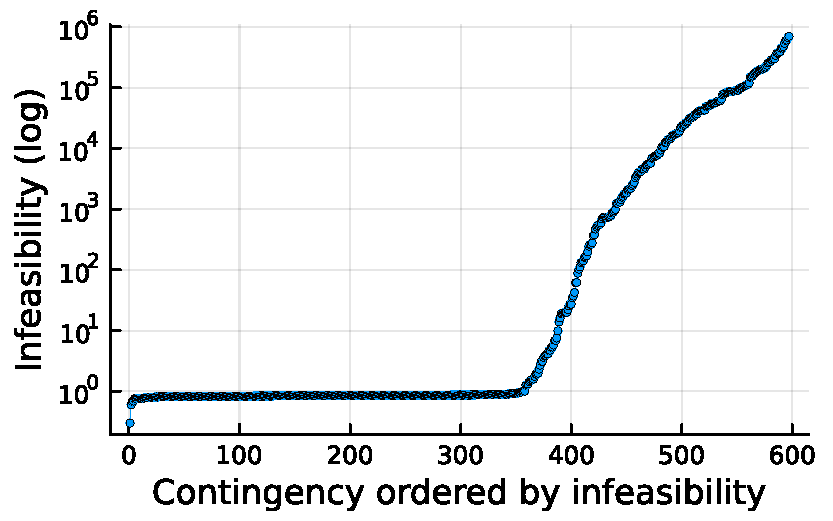
\includegraphics[width=.4\textwidth]{./figures/contingency.pdf}
\caption{Result of contingency screening for {\tt ACTIVSg500}.
The base case solution in \eqref{eq:screening} is obtained by solving
the classical OPF problem.}
\label{fig:contingency}
\end{figure}


\subsection{Solution of large-scale AC-SCOPFs on GPU}
\label{sec:numerics:scopf}
We are now in position to answer the main research question in this paper: is
MadNCL effective at solving large-scale AC-SCOPFs on the GPU?
We set up the following experiment.
We compare Knitro and MadNCL-CPU (using HSL MA57) with MadNCL-GPU (using NVIDIA cuDSS).
Knitro uses the modeler JuMP, which supports passing the complementarity constraints explicitly to the solver.
In contrast, MadNCL converts the JuMP model to ExaModels~\cite{shin2024accelerating} to benefit from faster evaluation
of derivatives (in particular on the GPU). MadNCL solves the NLP reformulation~\eqref{eq:mpccnlp}.
We select $K$ representative contingencies using the method described in \S\ref{sec:numerics:screening},
and ensure that all the contingencies are not structurally infeasible (so \eqref{eq:scopf} remains feasible).

First, we consider the case {\tt ACTIVSg500} and increase the number of contingencies
$K$ from $2$ to $256$ in \eqref{eq:scopf}: With $K=256$, the SCOPF~\eqref{eq:scopf} has almost 1 million variables.
We detail the results in Table~\ref{tab:scopfscalability}.
Interestingly, the number of iterations in MadNCL-CPU and MadNCL-GPU is different: as we enter the large-scale
regime, HSL MA57 and NVIDIA cuDSS are returning slightly different solutions, resulting in small discrepancies in the algorithm.
This is amplified by the parallel nature of NVIDIA cuDSS: consecutive runs in NVIDIA cuDSS can be non-deterministic for large $K$.
The objective value gives an insight on the quality of the solution: as the problem \eqref{eq:scopf} is nonconvex, different algorithms can converge
to different solutions. However, we observe that MadNCL-CPU and MadNCL-GPU both converge to the same solution as Knitro.
We show in Figure~\ref{fig:scalability} the time per iteration (in seconds) against
the number of contingencies for Knitro, MadNCL-CPU and MadNCL-GPU.
In term of raw performance, MadNCL-CPU is slightly faster than Knitro because MadNCL
benefits from faster evaluations of the derivatives with ExaModels (compared to JuMP).
MadNCL-GPU decreases the time per iteration further by at least an order of magnitude:
for $K \geq 64$, MadNCL-GPU becomes at least 20x faster than Knitro and 6x faster than MadNCL-CPU. The linear solver cuDSS here is
very effective at solving the linear system \eqref{eq:newtonsystem}, explaining the faster solution time on the GPU.

\begin{figure}[!ht]
\centering
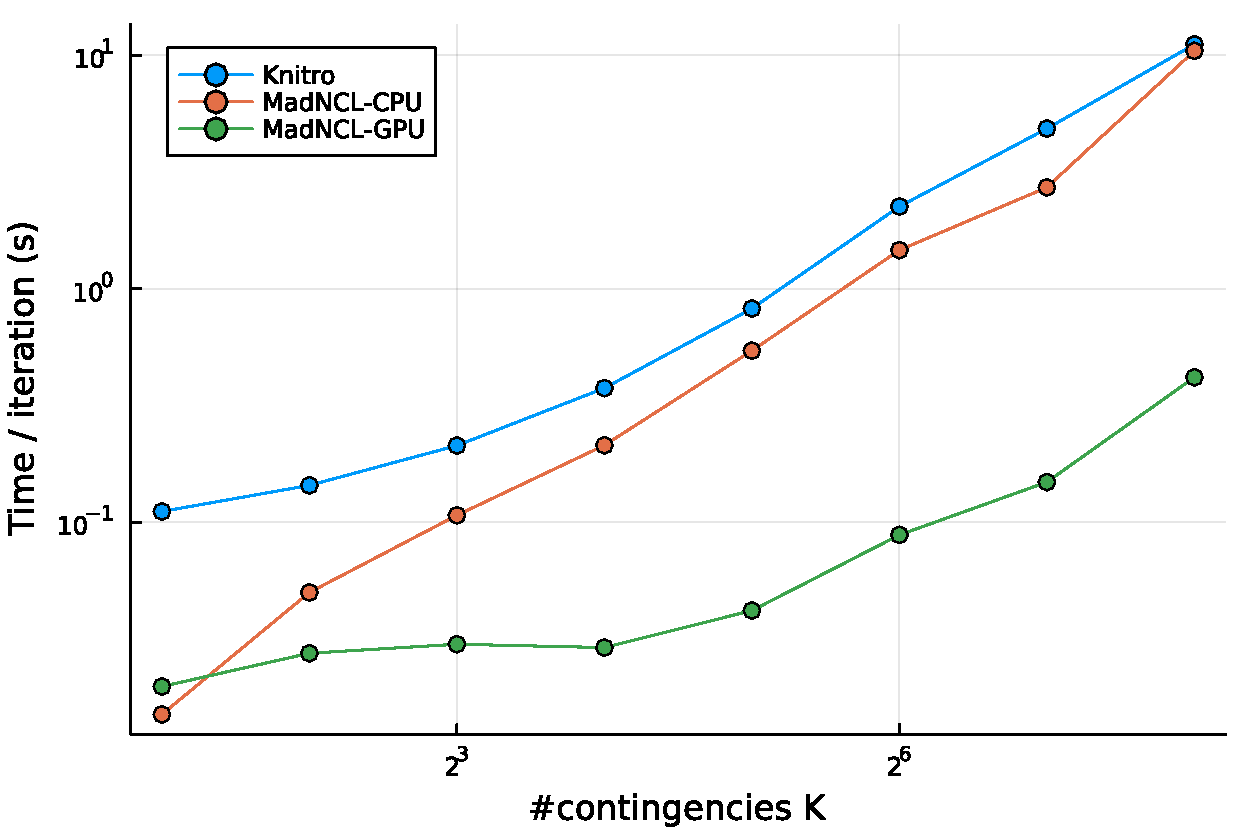
\includegraphics[width=.4\textwidth]{./figures/scalability.pdf}
\caption{Time per iteration (in seconds) against number of contingencies $K$
  when solving {\tt ACTIVSg500}. We compare Knitro (using JuMP)
against MadNCL (using ExaModels). We test MadNCL both on the CPU (using HSL MA57)
and on the GPU (using NVIDIA cuDSS).}
\label{fig:scalability}
\end{figure}

\begin{table*}[!ht]
\centering
\caption{Performance of Knitro and MadNCL as we increase the number
of contingencies $K$ for {\tt ACTIVSg500}. We display the total number of IPM iterations
and the time to solution (in seconds). The symbol "-" indicates that the solver failed
to find a solution.}
\resizebox{.95\textwidth}{!}{

\begin{tabular}{|r|rr|rrr|rrr|rrr|rrr|rrr|}
\hline
\multicolumn{ 3}{|c|}{}  & \multicolumn{ 3}{c|}{\bf Knitro (ref)} & \multicolumn{ 12}{c|}{\bf MadNCL} \\
\hline
\multicolumn{ 3}{|c|}{}  & \multicolumn{ 3}{c|}{JuMP+MA57 (CPU)} & \multicolumn{ 3}{c|}{JuMP+MA57 (CPU)} & \multicolumn{ 3}{c|}{SymbolicAD+MA57 (CPU)} & \multicolumn{ 3}{c|}{ExaModels+MA57 (CPU)} & \multicolumn{ 3}{c|}{ExaModels+cuDSS (GPU)}  \\
\hline
K & nvar & ncon
& Iter & Obj. & Time (s)& Iter & Obj. & Time (s)& Iter & Obj. & Time (s)& Iter & Obj. & Time (s)& Iter & Obj. & Time (s) \\
\hline
4 & 18k & 24k & 355 & 7.28 & 51.01 & 251 & 7.28 & 22.09 & 177 & 7.28 & 9.59 & 238 & 7.28 & 7.31 & 240 & 7.28 & 4.45\\
8 & 33k & 44k & 418 & 7.28 & 88.94 & 146 & 7.28 & 24.33 & 141 & 7.28 & 12.43 & 435 & 7.28 & 29.23 & 290 & 7.28 & 7.77\\
 16 & 63k & 83k & 114 & 7.28 & 42.76 & 180 & 7.28 & 58.50 & 199 & 7.28 & 38.39 & 214 & 7.28 & 25.71 & 261 & 7.28 & 6.65\\
 32 & 123k & 162k & 345 & 7.28 & 283.68 & 162 & 7.28 & 95.79 & 163 & 7.28 & 58.05 & 587 & 7.28 & 166.20 & 568 & 7.28 & 23.64\\
 64 & 242k & 319k & 960 & 7.28 & 2159.59 & 480 & 7.28 & 624.88 & 577 & 7.28 & 459.88 & 528 & 7.28 & 273.08 & 453 & 7.28 & 27.96\\
 128 & 480k & 634k & - & 7.29 & 4852.33 & 339 & 7.29 & 919.33 & 315 & 7.29 & 495.03 & 415 & 7.29 & 421.09 & 265 & 7.29 & 46.40\\
 256 & 957k & 1263k & - & 7.30 & 11136.08 & 700 & 7.30 & 4811.44 & 693 & 7.30 & 2976.29 & 493 & 7.30 & 1120.16 & 609 & 7.30 & 170.75\\
\hline
\end{tabular}

}
\label{tab:scopfscalability}
\end{table*}

Second, we compare Knitro and MadNCL-GPU on different instances, with a varying number of contingencies $K$.
The results are displayed in Table~\ref{tab:benchmark}.
We observe that MadNCL-GPU is consistently faster than Knitro. As in Table~\ref{tab:scopfscalability},
we do not have any guarantee that Knitro converges to the same solution as MadNCL: they
report a different solution for {\tt 1354pegase} and {\tt 2869pegase}.
We notice that MadNCL needs significantly more iterations
for {\tt ACTIVSg2000} and {\tt 2869pegase}. This points to MadNCL's main limitation:
as we increase the problem's dimension, we increase the degeneracy in the indefinite linear system~\eqref{eq:newtonsystem}.
As a result, the filter line-search algorithm used internally to solve Subproblem~\eqref{eq:nclsubpb} has to
perform numerous primal-dual regularizations during the inertia correction, significantly impairing MadNCL's convergence (we have observed that the ill-conditioning arises mostly from the reformulation
of \eqref{eq:pvpq}, when the reactive power lower-bound $\underline{q}_g$ is close to the upper-bound $\overline{q}_g$).
For that reason, we have observed that MadNCL does not converge consistently on larger instances.
We plan to address this issue in future work.


% An example is shown in Table~\ref{table_example}.
\begin{table*}[!ht]
% % increase table row spacing, adjust to taste
% \renewcommand{\arraystretch}{1.3}
\centering
\caption{Performance of Knitro and MadNCL-GPU on different instances. We
  display the total number of IPM iterations and the time to solution (in
  seconds). The symbol "-" indicates that the solver failed to find a solution.
}
\begin{tabular}{|rr|rr|rrr|rrr|}
\hline
\multicolumn{ 4}{|c|}{} & \multicolumn{ 3}{c|}{\bf Knitro} & \multicolumn{3}{c|}{\bf MadNCL-GPU} \\
\hline
Name        & K   & nvar   & ncon   &  Iter & Obj. & Time (s) &  Iter & Obj. & Time (s) \\
\hline
ACTIVSg200  & 10  & 17546  & 22841  &  141  & 2.76      & 14.84    &  34   & 2.76      & 3.48     \\
ACTIVSg200  & 50  & 81906  & 106721 &  147  & 2.76      & 106.99   &  52   & 2.76      & 2.63     \\
ACTIVSg200  & 100 & 162356 & 211571 &  81   & 2.76      & 97.93    &  49   & 2.76      & 3.00     \\
\hline
ACTIVSg500  & 10  & 40750  & 53753  &  290  & 7.47      & 82.27    &  70   & 7.37      & 2.78     \\
ACTIVSg500  & 50  & 189750 & 250433 &  533  & 7.83      & 871.45   &  257  & 7.76      & 39.65    \\
ACTIVSg500  & 100 & 376000 & 496283 &  294  & 7.83      & 935.19   &  131  & 7.76      & 17.80    \\
\hline
1354pegase  & 8   & 109056 & 144327 &  43   & 7.41      & 53.82    &  36   & 7.43      & 5.08     \\
1354pegase  & 16  & 206920 & 273999 &  30   & 7.41      & 86.90    &  39   & 7.43      & 4.81     \\
1354pegase  & 32  & 402648 & 533343 &  116  & 7.41      & 656.68   &  57   & 7.41      & 12.64    \\
\hline
ACTIVSg2000 & 8   & 173024 & 229853 &  160  & 122.89    & 1442.62  &  -    & -         & -        \\
ACTIVSg2000 & 16  & 328360 & 436469 &  141  & 122.89    & 3001.10  &  747  & 122.89    & 143.28   \\
\hline
2869pegase  & 8   & 242102 & 323479 &  65   & 13.40     & 308.77   &  45   & 13.44     & 5.94     \\
2869pegase  & 16  & 459118 & 613727 &  68   & 13.40     & 775.95   &  348  & 13.40     & 75.71    \\
\hline
\end{tabular}

\label{tab:benchmark}
\end{table*}

\section{Conclusion}

In this article, we have studied the solution of large-scale AC-SCOPFs
using MadNCL, a GPU-accelerated solver. As illustrated by Figure~\ref{fig:scalability},
MadNCL is significantly faster on the GPU than a similar solver running on the CPU,
with a time per iteration decreased by a factor of almost 40 on the largest instances.
As a result, MadNCL can find in less than 3 minutes a strongly stationary solution for AC-SCOPFs with almost a million decision variables, allowing instances with thousands of buses and
hundred of contingencies to be tackled. In future work, we plan to move the threshold further:
this would require addressing the ill-conditioning appearing in the IPM's Newton systems,
caused by the millions of complementarity constraints found in AC-SCOPF with
more than 10,000 buses and 100 contingencies.

\section*{Acknowledgements}
We thank Michael Saunders for giving us a thorough feedback on the first version
of this paper. We also thank the three anonymous reviewers for their valuable remarks.

% \subsection{Figures}
% An example of a floating figure using the graphicx package.
% Note that \label must occur AFTER (or within) \caption.
% For figures, \caption should occur after the \includegraphics.
% Note that IEEEtran v1.7 and later has special internal code that
% is designed to preserve the operation of \label within \caption
% even when the captionsoff option is in effect. However, because
% of issues like this, it may be the safest practice to put all your
% \label just after \caption rather than within \caption{}.
%
%

% Note that IEEE typically puts floats only at the top, even when this
% results in a large percentage of a column being occupied by floats.


% An example of a double column floating figure using two subfigures.
% (The subfig.sty package must be loaded for this to work.)
% The subfigure \label commands are set within each subfloat command,
% and the \label for the overall figure must come after \caption.
% \hfil is used as a separator to get equal spacing.
% Watch out that the combined width of all the subfigures on a
% line do not exceed the text width or a line break will occur.
%
%\begin{figure*}[!t]
%\centering
%\subfloat[Case I]{\includegraphics[width=2.5in]{box}%
%\label{fig_first_case}}
%\hfil
%\subfloat[Case II]{\includegraphics[width=2.5in]{box}%
%\label{fig_second_case}}
%\caption{Simulation results for the network.}
%\label{fig_sim}
%\end{figure*}
%
% Note that often IEEE papers with subfigures do not employ subfigure
% captions (using the optional argument to \subfloat[]), but instead will
% reference/describe all of them (a), (b), etc., within the main caption.
% Be aware that for subfig.sty to generate the (a), (b), etc., subfigure
% labels, the optional argument to \subfloat must be present. If a
% subcaption is not desired, just leave its contents blank,
% e.g., \subfloat[].





% trigger a \newpage just before the given reference
% number - used to balance the columns on the last page
% adjust value as needed - may need to be readjusted if
% the document is modified later
%\IEEEtriggeratref{8}
% The 'triggered' command can be changed if desired:
%\IEEEtriggercmd{\enlargethispage{-5in}}

% references section

% can use a bibliography generated by BibTeX as a .bbl file
% BibTeX documentation can be easily obtained at:
% http://www.ctan.org/tex-archive/biblio/bibtex/contrib/doc/
% The IEEEtran BibTeX style support page is at:
% http://www.michaelshell.org/tex/ieeetran/bibtex/
% argument is your BibTeX string definitions and bibliography database(s)
%\bibliography{IEEEabrv,../bib/paper}
%
% <OR> manually copy in the resultant .bbl file
% set second argument of \begin to the number of references
% (used to reserve space for the reference number labels box)
% \begin{thebibliography}{1}
% \bibitem{Shell}
% M.~Shell, \emph{How to Use the IEEEtran Latex Class}, Latex Archive Contents, \verb+http://www.ieee.org/conferences_events/+ \verb+conferences/publishing/templates.htm+

% \bibitem{IEEEhowto:kopka}
% H.~Kopka and P.~W. Daly, \emph{A Guide to \LaTeX}, 3rd~ed.\hskip 1em plus
%   0.5em minus 0.4em\relax Harlow, England: Addison-Wesley, 1999.




% \end{thebibliography}

\bibliographystyle{IEEEtran}
\bibliography{IEEEabrv,biblio.bib}


% that's all folks
\end{document}


